Justificación de las técnicas y tecnologías empleadas en el trabajo, especificando las razones por las que se han descartado otras igualmente aplicables.

\section{Metodología}

En este apartado se especificarán las fases del trabajo, así como la metodología o metodologías empleadas para desarrollar cada una de las fases. 

\newpage

\section{Tecnologías empleadas}

Las tecnologías utilizadas para el desarrollo de la aplicación se pueden clasificar según su uso. Debido a que el formato propuesto para el desarrollo es similar al de un videojuego, donde la interacción es esencial para su uso correcto y óptimo, se ha seleccionado software adecuado para el producto realizado. A continuación, se explicará detalladamente el uso de las diferentes tecnologías y las razones detrás de la elección de cada una específicamente.

\subsection{Unity}

Un motor de videojuegos, del inglés game engine, es un entorno que proporciona un conjunto de herramientas reutilizables que facilitan la creación de videojuegos a los desarrolladores. Estos se pueden dividir en el motor gráfico, responsable del aspecto visual, y el motor físico, encargado de dotar al motor de leyes físicas como la gravedad, la masa o las fuerzas. Cada motor de videojuegos tiene sus propios usos y limitaciones. Por lo tanto, la elección del motor a utilizar es de gran importancia antes de iniciar el desarrollo. Existen motores más especializados en el desarrollo 3D como \textit{Unreal Engine} (\cite{UE:1998}), mientras que otros están centrados en gráficos 2D, como \textit{Game Maker Studio} (\cite{GMS:1999}) y \textit{RPG Maker} (\cite{RPGM:1992}). \textit{Unity} (\cite{UNITY:2005}) y \textit{Godot Engine} (\cite{GODOT:2001}) son híbridos que permiten el desarrollo en ambas dimensiones.

Unity, junto con Unreal Engine y recientemente Godot Engine, es uno de los motores de videojuegos más populares en la industria. Aunque Unreal Engine es valorado como posiblemente el mejor motor de videojuegos de la actualidad, su uso está limitado a circunstancias muy específicas: videojuegos 3D para consolas de última generación. Sin embargo, Unity, aunque no ofrece la potencia gráfica de Unreal Engine, es mucho más versátil y se puede utilizar en una amplia variedad de circunstancias. Esto permite que el rango de plataformas para las que se puede desarrollar con este motor aumente, convirtiéndolo en una opción más segura para enfocarse en el desarrollo multiplataforma.

\begin{figure}[h!]
	\centering
	\subfigure[Unity.]{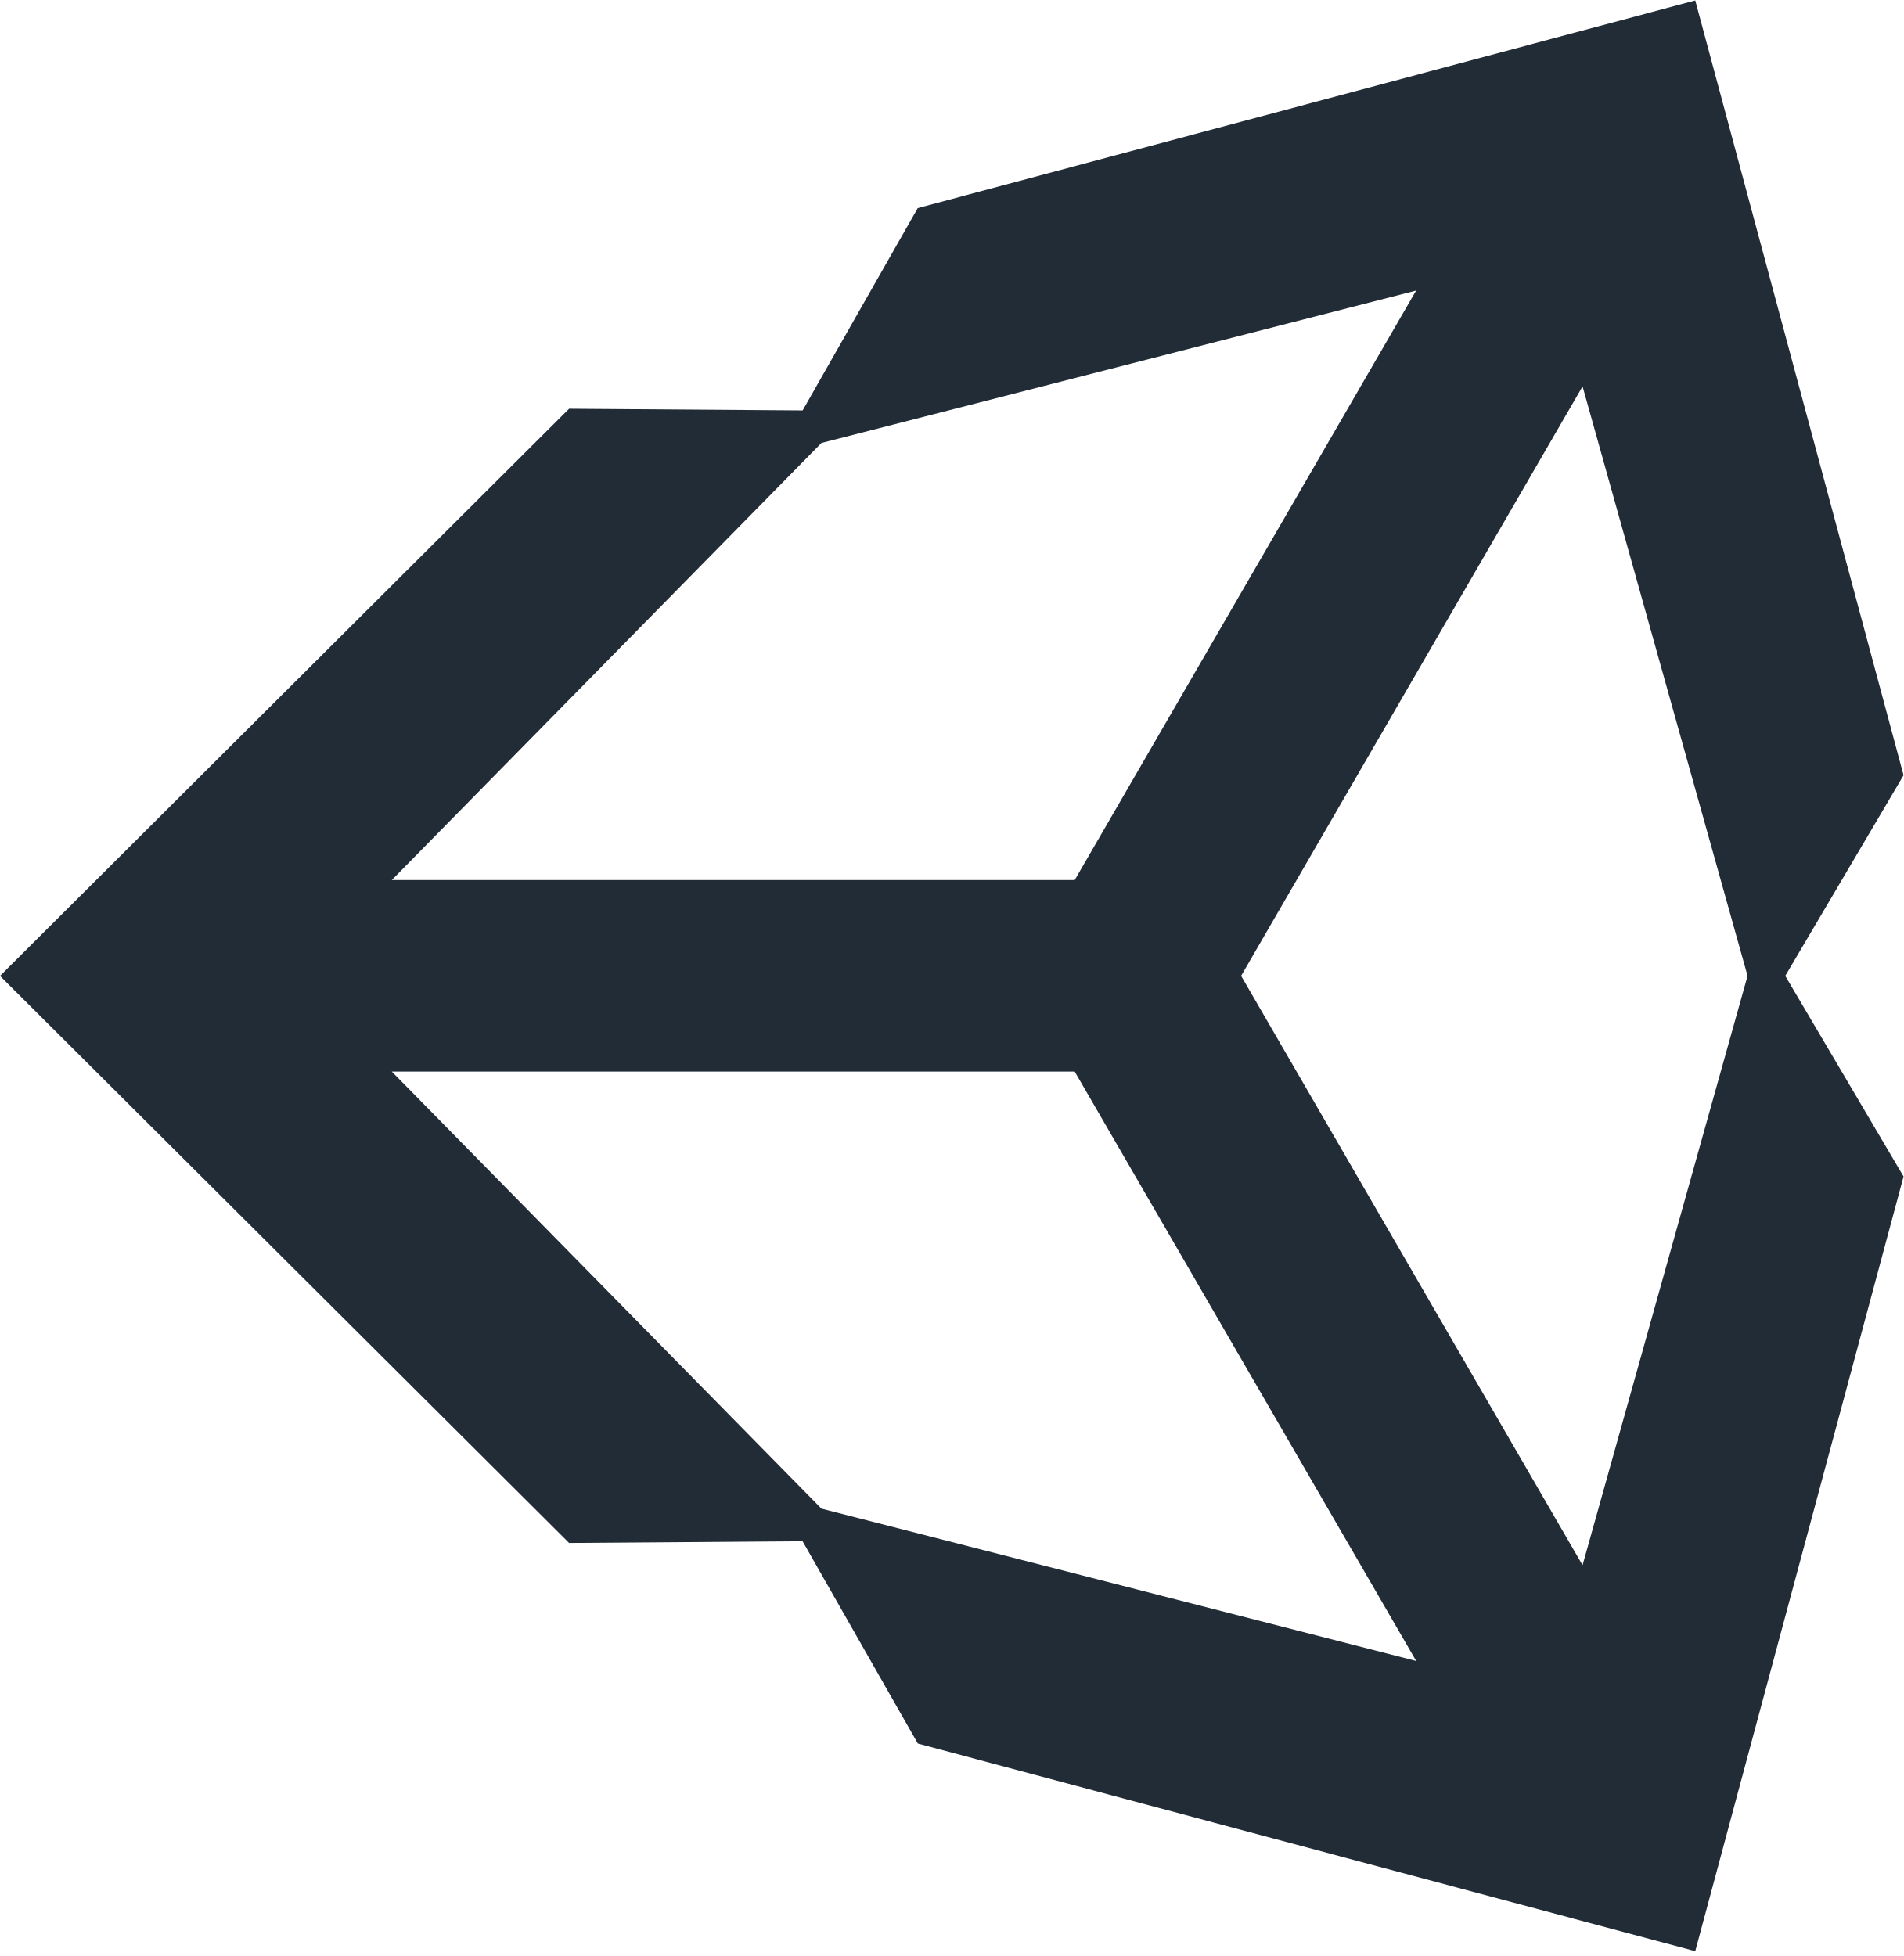
\includegraphics[width=0.2\textwidth]{./Figuras/Aspectos/UnityLogo}\label{fig:UnityLogo}}
	\hfil
	\subfigure[Unreal Engine.]{
\includegraphics[width=0.2\textwidth]{./Figuras/Aspectos/UnrealLogo.png}\label{fig:UnrealLogo}}
	\hfil
	\subfigure[Godot Engine.]{
\includegraphics[width=0.2\textwidth]{./Figuras/Aspectos/GodotLogo.png}\label{fig:GodotLogo}}
	\caption{Logotipos de los motores de videojuegos mencionados en el párrafo anterior.}
	\label{fig:GameEngineLogos}
\end{figure}

En nuestro caso, elegimos Unity por varias razones. Nuestra plataforma objetivo son dispositivos móviles, específicamente tabletas. Unity domina el 50\% del desarrollo de videojuegos para plataformas móviles, consolas y PC. Además, el 71\% de los 1000 mejores videojuegos móviles están realizados en Unity (\cite{PLARIUM:2024}).

\subsection{FMOD}

\subsection{TeXstudio}

\subsection{Adobe Illustrator?}